\documentclass{article}

%%%%%%% PACKAGES %%%%%%%%
\usepackage[utf8]{inputenc}
\usepackage[margin=2cm]{geometry}
\usepackage{blindtext}
\usepackage{setspace}
\usepackage{graphicx}
\usepackage{notoccite} %citation number ordering
\usepackage{lscape} %landscape table
\usepackage{caption} %add a newline in the table caption
\usepackage{color}
\usepackage[dvipsnames]{xcolor}
\definecolor{ultramarine}{HTML}{2f3973}
\definecolor{hexablack}{HTML}{000000}
\usepackage[colorlinks = true,
linkcolor = hexablack,
urlcolor  = ultramarine,
citecolor = ultramarine,
anchorcolor = hexablack]{hyperref}

\title{\huge{\textbf{Gesture Based UI Development}} \\
\LARGE{Research Paper}}
\author{John Shields}
\date{February 2021}

\begin{document}
\pagenumbering{roman} % Start roman numbering
\clearpage\maketitle
\thispagestyle{empty}
\begin{center}
    \begin{figure}[h]
        \centering
        
\includegraphics[width=15cm]{pics/logo-gmit.png}
        %\caption{Your caption here}
        \label{fig:logo}
    \end{figure}
    \large{	BSc (Hons) in Software Development \\
    Lecturer: Damien Costello}
\end{center}
\newpage
\setcounter{page}{1}
\tableofcontents
\listoffigures

\newpage
\pagenumbering{arabic} % Start roman numbering

%%% CONTENT START HERE %%%%
\section{Description}
This Research Paper is based on Gesture Based User Interface Experience that focuses on Accessibility, Evolution and Challenges. The purpose of this paper is to research the User Interface as it moves from purely physical (mouse, keyboard, touch screen) to include intuitive interaction through gestures.

\section{Introduction}
Gesture Based User Interface Experience can vary in many ways. Computers are all around us. It can be said that almost every household has at least one computer, where it be a PC or a Laptop, there is sure to be one in most homes today. Obviously, computers are not the only devices in homes. Nowadays, Phones are extremely popular and heavily used. They might even be used more than computers. Having said that, a phone is basically a computer that you can fit in your pocket. Gesture Based UI is heavily used in these devices. For a computer, this can be as simple as sliding your hand to the left and right to go back and forth between pages. Gestured Based UI only came into play with phones when the touch screen was introduced. Computer too can have touch screens, but it is optional. Most personal phones likely have touch screens. Today's phones rely on the touch screen. They only have a few physical buttons. These are mainly for locking/unlocking phones and for adjusting the volume level. Gesture Based UI is not just for computers and phones. It is also for something as simple as a watch or a car radio, making them all the smarter. Gestured Based UI makes every device smarter.

\section{User Experience Evolution}
User Experience is constantly Evolving. The first general-purpose computer was the monolithic ENIAC machine. The machine's construction began on the 13th of May, 1943, and was finished on the 2nd of October, 1955. The User Experience on the ENIAC was a bit of a headache and relied on many experts to work the machine. ENIAC was designed to be capable of being reprogrammed to solve a large number of numerical problems. The machine's programming consisted of setting switches and connecting wires according to specific instructions, which were first worked out on paper, which took weeks. This machine also used a punch-card reader as an input and output device. This is obviously not very user-friendly, but for the time, it was extraordinary. Comparing this machine to any computer or smart device today shows how much these technologies have evolved. \cite{ref1}

\begin{figure}[h!]
    \caption{ENIAC Machine \cite{ref2}}
    \label{image:ENIAC}
    \centering
    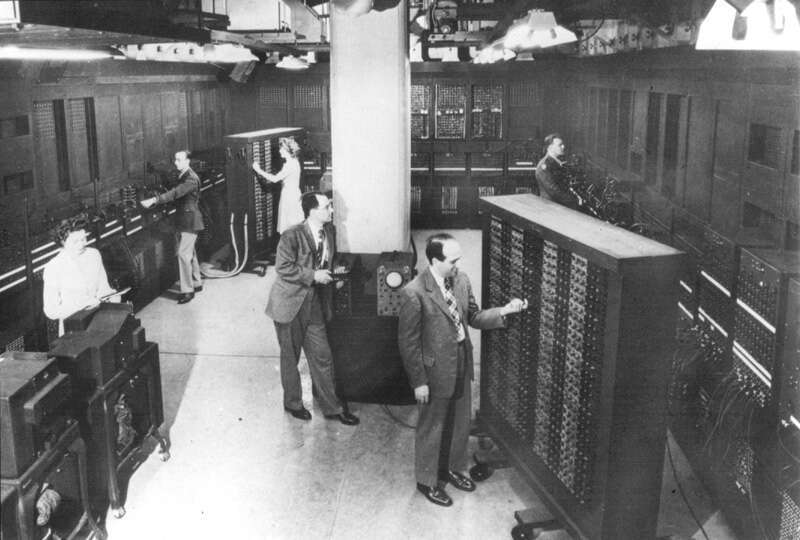
\includegraphics[width=0.5\textwidth]{pics/eniac.jpg}
\end{figure}

One of the key parts of a computer that is still highly used today is the keyboard. Keyboards are inspired by typewriters. The typewriter has been around since the late 1800s and is an antique that is still used today. The QWERTY keyboard layout, which came from the Sholes and Glidden typewriter, also came from this time. QWERTY's design has the keys to be spread out to avoid jamming those old typewriters. The QWERTY layout remains to be very popular in the English speaking world. The Binac computer (1948) used an electromechanically controlled typewriter to input data directly onto magnetic tape and print results. This was the first integration of a keyboard like system for a computer. \cite{ref3}

\begin{figure}[h!]
    \caption{The Binac Computer \cite{ref4}}
    \label{image:BINAC}
    \centering
    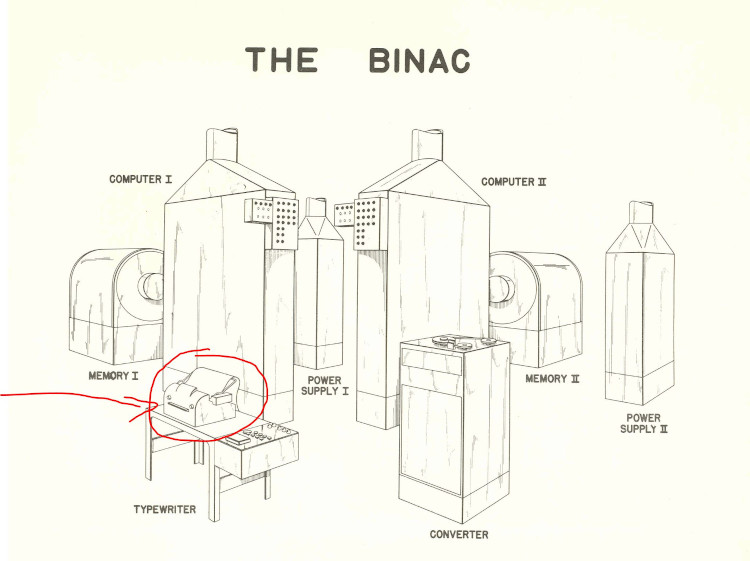
\includegraphics[width=0.5\textwidth]{pics/binac.jpg}
\end{figure}


\section{Gestures as a communication tool}

\section{Challenges for design of applications}

\section{Challenges for implementation}

\section{Conclusions}

 \newpage
 \begin{thebibliography}{00}
    
\bibitem{ref1} History of Computers
\newline
URL: \url{https://homepage.cs.uri.edu/faculty/wolfe/book/Readings/Reading03.htm}

\bibitem{ref2} SUZANNE DEFFREE - EDN - Construction begins on ENIAC
\newline
URL: \url{https://www.edn.com/construction-begins-on-eniac-may-31-1943/}

\bibitem{ref3} Mary Bellis - The History of the Computer Keyboard
\newline
URL: \url{https://www.thoughtco.com/history-of-the-computer-keyboard-1991402}

\bibitem{ref4} The Binac Computer
\newline
URL: \url{https://tinyurl.com/y266fydp}

\end{thebibliography}

%%% CONTENT HERE END %%%%
\end{document}
\newpage
\setstretch{1}  %reduce bibliography line spacing
\printbibliography
\end{document}